\documentclass{beamer}
\usepackage{graphicx}
\begin{document}
\begin{frame}
\begin{center}
STORM WATER MANAGEMENT AND DRAINAGE  MAINTENANCE  SYSTEM  USING  IOT
\end{center}
\end{frame}
\begin{frame}
\frametitle{PROBLEM DOMAIN}
\begin{itemize}
\item Clean water and sanitation.
\item Drainage stagnate level indication.
\end{itemize}
\end{frame}
\begin{frame}
\frametitle{HOW MIGHT WE ?}
Drainage stagnate level intimation during heavy downpour of rain which solves the issues of traffic, contagious diseases and problems of sewage for public.
\end{frame}
\begin{frame}
\frametitle{CAUSES AND EFFECTS}
\textbf{causes}
\begin{enumerate}
\item Heavy downpour in metros
\item Much of water stagnation
\item Poor drainage system
\end{enumerate} 
\textbf{effects}
\begin{enumerate}


\item Poorly maintained drains will cause flooding which causes enormous   
  damages in the agricultural land and irrigation network
\item Spread of diseases
\item Water logging in agricultural fields
\end{enumerate}
\end{frame}
\begin{frame}
\begin{itemize}
\frametitle{STAKEHOLDER}
\item Roles of responsibilities of government bodies relating to drainage and  flood regulation
\end{itemize}
\end{frame}
\begin{frame}
\frametitle{KEY PERFORMANCE INDICATORS}
\begin{enumerate}
\item Arduino IDE.
\item Microcontroller board.
\item Wifi module.
\item Flow sensors.
\item Water level sensors.
\end{enumerate}
\end{frame}
\begin{frame}
\frametitle{CUSTOMER AND MARKET RESEARCH}
\begin{enumerate}
\item Global stormwater management market is projected to grow at a CAGR of 8.8\%  by 2023, on the back of increasing number of intense floods and storms coupled with rising urbanization.
\item Increase in the number and intensity of landslides due to heavy storm, snow and rainfall drive the adoption of stormwater management solutions for efficient water management and sustainable infrastructure development.
\end{enumerate}
\end{frame}
\begin{frame}
\frametitle{ATOMIC UNIT}
\begin{itemize}
\item Locating the exact position of water stagnate.
\item Intimating the concerned municipality officer about the status of  
 water stagnate levels.
\end{itemize}
\end{frame}
\begin{frame}
\frametitle{BLOCK DIAGRAM}
\begin{center}
\begin{figure}
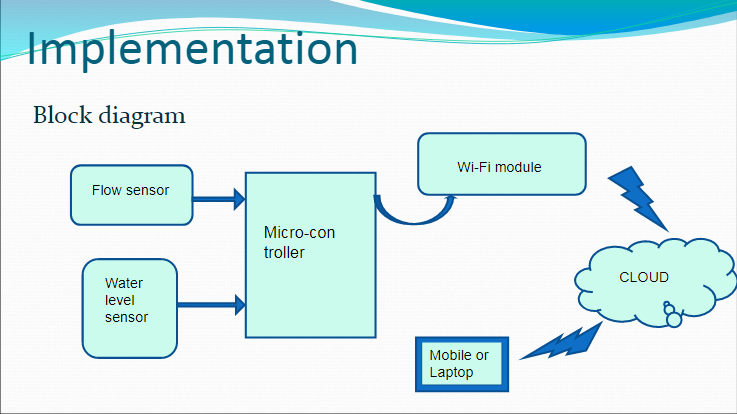
\includegraphics[width=10cm,height=6cm]{456}
\end{figure}
\end{center}
\end{frame}
\begin{frame}
\begin{center}
THANK YOU
\end{center}
\end{frame}
\end{document}


